\documentclass{standalone}
\usepackage{tikz}

\begin{document}
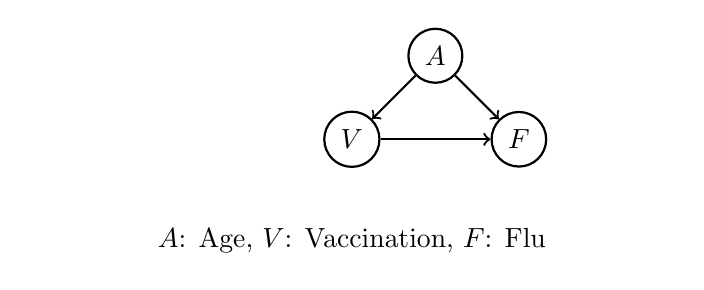
\begin{tikzpicture}[node distance={15mm}, thick, main/.style = {draw, circle}]
    \node[main] (1) {$A$};
    \node[main] (2) [below left of=1] {$V$};
    \node[main] (3) [below right of=1] {$F$};

    \draw[->] (1) -- (2);
    \draw[->] (1) -- (3);
    \draw[->] (2) -- (3);

    \node [below=1cm, align=flush center,text width=8cm] at (2)
        {
            $A$: Age, $V$: Vaccination, $F$: Flu
        };

    \end{tikzpicture}
\end{document}
